%!TEX root = ../document.tex
\chapter{Lösungsansatz} \label{chp:Loesungsansatz}
	In diesem Kapitel wird ein Verfahren zur Georeferenzierung von Twitter-Nutzern vorgestellt.
	Die Fragestellungen aus Kapitel \ref{sec:fragestellung} werden, unter Berücksichtigung der Anforderungen aus Kapitel \ref{sec:Anforderungen}, beantwortet.  

	Zunächst soll ein Überblick über die Funktion und den Ablauf des Verfahrens gegeben werden ohne detailliert auf die einzelnen Verfahrensschritte einzugehen.
	Danach soll eine generelle Struktur einer Georeferenz-Basis zur Georeferenzierung vorgestellt werden.
	In den darauffolgenden Abschnitten wird ganz allgemein betrachtet anhand welcher Indikatoren eine Georeferezierung möglich ist, bevor die möglichen Indikatoren aus Twitter betrachtet werden.
	Basierend darauf soll dann ein Verfahren zum einlernen der Georeferenz-Basis erarbeitet werden.
	Dabei wird auch die Struktur der Georeferenz-Basis angepasst um die Anforderungen zu erfüllen.
	Zum Schluss wird ein Verfahren zur Georeferezierung mit Hilfe der Georeferenz-Basis am Beispiel von Twitter vorgestellt.
	Es wird ein Analyseverfahren vorgestellt, das es ermöglicht Konfidenzen zu einer Georeferenz anzugeben.
	Des weiteren wird gezeigt wie die geografische Hierarchie bei der Georeferenzierung ausgenutzt werden kann. 


	\section{Überblick} \label{sec:ueberblick} 
		Das erarbeitete Verfahren soll es ermöglichen Twitter-Nutzern eine Georeferenz zuzuordnen.
		Dabei sollen als Eingabe für die Georeferenzierung lediglich der Nutzer-Standort und die Nutzer-Zeitzone aus dem Profil eines Twitter-Nutzers verwendet werden.
		Als Ergebnis soll eine Georeferenz mit einem Konfidenzwert zurückgeliefert werden. 
		Dabei hat der Anwender die Möglichkeit einen Schwellwert für die Konfidenz anzugeben.
		Zudem kann der Nutzer die gewüschte Hierarchiebene angeben derer der Rückgabewert entsprechen soll. 
		In Abbildung \ref{img:GeoreferenzierungAllg} ist der generelle Ablauf dieser Georeferenzierung dargestellt. 
		\todo{Schema Darstellung Eingabe->Ausgabe  Sketchbook A1: Unterschrift Die Eingabe besteht aus dem Nutzer-Standort sowie der Nutzer-Zeitzone. 
		Als Rahmenbedingungen wird die gewünschte Hierarchieebene sowie der Schwellwert für die Konfidenz angeben. 
		Als Ausgabe erhält man eine Georeferenz} 

		\begin{figure}[h!]
			\begin{center}
				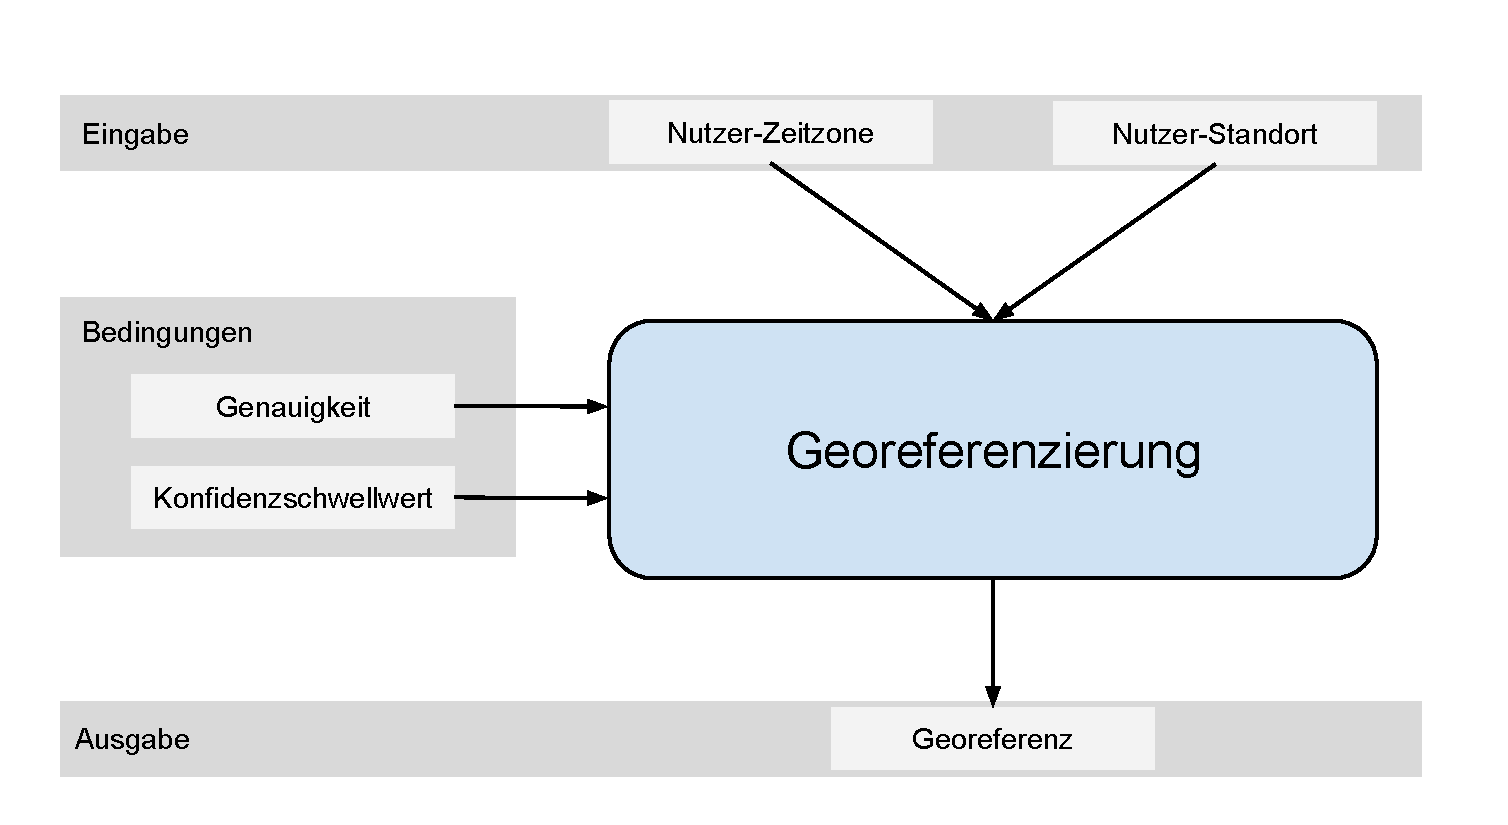
\includegraphics[scale=0.5]{A1.pdf}
				\caption{Ablauf Georeferenzierung}
				\label{img:georef}
			\end{center}
		\end{figure}	

		Die Georeferenzierung nach dem Schema aus Abbildung \ref{img:georef} setzt voraus, dass aus den eingegebenen Indikatoren eine Georeferenz abgeleitet werden kann.     
		Dies ist mit einer Datenbasis, die zu einem gegebenen Indikator eine Georeferenz liefern kann möglich.
		Aus einer Tweet-Datensammlung soll die Zuordnung der Indikatoren zu geografischen Positionen gelernt werden.
		Diese gelernten Zuordnungen sollen in einer Datenbasis gespeichert werden.
		Diese Datenbasis wird Georeferenz-Basis genannt.
		
		Zur Erstellung der Georeferenz-Basis werden zunächst einige Schritte zur Vorverarbeitung der Indikatoren durchgeführt.
		Zusätzlich wird die in jedem Tweet anegegebene Georeferenz verarbeitet.
		In der Georeferenz-Basis werden nun die so erstellen Indikator-Werte mit den entsprechenden Georeferenzen gespeichert.
		Der generelle Ablauf zur Erstellung der Georeferenz-Basis wird in Abbildung \ref{img:ablaufEinlernen} dargestellt.

		Bei der Georeferenzierung werden die Indikatoren zunächst derselben Vorverarbeitung wie beim einlernen unterzogen.
		Die Vorverarbeitungsschritte sind somit generisch, da sie sowohl vor dem erzeugen der Georeferenz-Basis als auch vor der eigentlichen Georeferenzierung durchgeführt werden.
		Nach der Vorverarbeitung werden die Indikatoren in der Georeferenz-Basis nachgeschlagen.
		Das Ergebnis ist eine Menge aus Indikatoren und zugehörigen Georeferenzen. 
		Durch eine Analyse der Ergebnisse kann dann eine Georeferenz zugewiesen werden.
		Der Ablauf der Georeferenzierung wird in Abbildung \ref{img:Georeferenzierung} dargestellt. 

		\todo{img:georef, img:ablaufEinlernen, img:Georeferenzierung} 

		In den folgenden Kapiteln sollen die Probleme der Georeferenzeirung in Hinblick auf Twitter betrachtet werden. 
		Dabei werden Toponyme genauer betrachtet und an einigen Beispielen die Problematik des Nutzer-Standortes aus Twitter erläutert.
		Basierend darauf soll ein Verfahren zum einlernen der Georeferent-Basis und eine Struktur für die Georeferenz-Basus entwickelt werden.
		Im letzten Kapitel wird die Georeferenzierung betrachtet.
		Mit Hilfe eines Analyseverfahrens sollen die Probleme bei der Verwendung des Nutzer-Standortes und der Nutzer-Zeitzone behoben werden.

	\section{Generelle Struktur einer Georeferenz-Basis zur Georeferenzierung} \label{sec:generelleStruktur} 

		In diesem Kapitel soll eine generelle Struktur angegeben werden, welche die minimalen Anforderungen einer Georeferenzierung erfüllen kann.
		Danach wird das Schema und die nötigen Informationen, welche die Georeferenz-Basis beinhaltet, genauer betrachtet.
		
		Nach Abbildung \ref{img:allgA1} wird durch die Georeferenzierung einer Menge geografischer Indikatoren eine Georeferenz zugewiesen.
		In der einfachsten Variante wird lediglich ein einziger geografischer Indikator an die Georeferenzierung übergeben und genau eine Georeferenz zurückgegeben.
		Die Georeferenzierung muss also zu einem gegebenen geografischen Indikator eine Georeferenz bestimmen können.
		Dies führt zu einer ersten einfachen Struktur für die Georeferenz-Basis.	

		\subsection*{Eine erste einfache Struktur der Georeferenz-Basis} 

			Es wird angenommen der geografische Indikator stellt immer ein eindeutiges Toponym dar.
			Des weiteren sind alle möglichen Toponyme sowie eine zugehörige Georeferenz bekannt. 
			Die Georeferenz liegt als Adresse mit Straße, Hausnummer, Postleitzahl und Ortsname vor.

			Jedem möglichen Toponym, welches im gegebenen geografischen Indikator vorkommen kann, soll eine Georeferenz zugeordnet werden können. 
			Daraus ergibt sich die Anforderung, dass die Georeferenz-Basis eine Menge von Datensätzen beinhalten muss, die jeweils aus einem Toponym und einer Georeferenz bestehen.
			Dieser Aufbau entspricht einer Art Wörterbuch in dem Informationen zu einem gegebenen Referenzwert nachgeschlagen werden können.
			Im vorliegenden Fall kann also zu einem Toponym die enstprechende Georeferenz nachgeschlagen werden.
			Die Referenzwerte stellen dabei mögliche Werte für die Indikatoren dar. 
			In Abbildung \ref{tab:simpleStruktur} ist ein Beispiel für eine sehr simplen Struktur dargestellt.

			\begin{table}[htpb]
					\caption{Erste einfache Struktur für eine Georeferenz-Basis zur Georeferenzierung} 
					\centering
					\begin{tabular}{|c|c|}
						\hline
						Referenzwert & Georeferenz \\
						\hline\hline
						Zoo-Karlsruhe & Ettlinger Straße 6 - 76137 Karlsruhe \\
						\hline
						ZKM & Lorenzstraße 19 D - 76135 Karlsruhe \\
						\hline
						Elbphilharmonie & Dammtorwall 46 - 20355 Hamburg \\
						\hline
					\end{tabular}
					\label{tab:simpleStruktur} 
			\end{table} 

			Wird eine Abfrage auf die Georeferenz-Basis mit den Indikatoren "'Zoo-Karlsruhe"', "'ZKM"' oder "'Elbphilharmonie"' durchgeführt, kann nun eine Georeferenz zurückgeliefert werden.
			Diese simple Struktur reicht grundsätzlich aus um eine Georeferenzierungen durchführen zu können.
			In dem angeführten Beispiel ist die Menge der möglichen Toponyme sehr begrenzt, aber diese kann beliebig erweitert werden.
			Damit können sehr mächtige Datenbanken erstellt werden.

			Es sollen nun der Referenzwert und die Georeferenz genauer betrachtet werden.

			\paragraph{Form der Georeferenz}

				Die Form in der die Georeferenz angegeben wird ist abhängig von der Anwendung. 
				Im Beispiel \ref{tab:simpleStruktur} wurden Adressen verwendet. 
				Dazu muss das angegebene Toponym oder die Zeichenkette jedoch eine Adresse besitzen. 
				Ein See in der Wildnis Alaskas wird keine solche Adresse aufweisen.
				Aber auch die geografische Position einer Stadt oder eines Landes kann nicht durch eine Adresse beschrieben werden. 
				Die Form in der die Georeferenz angegeben wird kommt auf den jeweiligen Anwendungsfall an.
				Denkbar sind hier unter anderem:

				\begin{itemize}
				  	 \item geografische Koordinaten
				  	 \item vollständige Adressen
				  	 \item Länder
				  	 \item Städte
				  	 \item adminsitrative Verwaltungsgebiete 
				  	 \item Zeitzonen
				  	 \item Straßenname und eine Kilometerbezeichnung
				  \end{itemize}  

				  Grundsätzlich sind alle Formen, welche eine direkte oder indirekte Georeferenz darstellen, denkbar.
				  Wichtig ist nur, dass die Angabe der Georeferenz in einer Form erfolgt welche für die gegebene Anwendung ausreichend genau ist.

				  Für den Straßenverkehr ist eine Angabe einer Adresse ausreichend.
				  Für Wanderungen in unerschlossenen Gebieten hingegen sind geografische Koordinaten notwendig. 

			\paragraph{Form der Referenzwerte}

				Der Referenzwert ergibt sich aus den möglichen Werten der Indikatoren.
				Die Indikatoren sind dabei zumeist Zeichenketten.
				Abhängig vom Indikator können diese Zeichenketten verschiedene Informationen enthalten.
				Im obigen Beispiel sind die Referenzwerte Toponyme.
				Toponyme sind Namen für geografische Objekte, es kann ihnen also unmittelbar ein geografische Objekt zugeordnet werden.
				Es muss sich dabei aber nicht um Toponyme handeln.
				Werte die als Referenzwerte in Frage kommen sollen als geografische Indikatoren bezeichnet werden.
				Toponyme sind also geografische Indikatoren, da sie direkt mit einem geografischen Objekt in Verbindung gebracht werden können.
				Geografische Indikatoren können aber auch indirekt mit einem geografischen Objekt in Verbindug gebracht werden.
				Unbrauchbar sind Werte welche weder direkt noch indirekt mit einem geografischen Objekt in Verbindung gebracht werden können.
				Diese Werte stellen keine geografischen Indikatoren dar.
				Im nächsten Abschnitt werden die geografischen Indikatoren genauer betrachtet.

	\section{Geografische Indikatoren} 

		Geografische Indikatoren sind diejenigen Indikatoren welche einen geografischen Bezug aufweisen.
		Es sind also genau die Werte, welche in irgendeiner Weise mit einem geografischen Objekt in Verbindung gebracht werden können.

		Geografische Indikatoren lassen sich in unmittelbare geografische Indikatoren und mittelbare geografische Indikatoren aufteilen. 
		In diesem Abschnitt soll sowohl auf die unmittelbaren wie auch die mittelbaren geografischen Indikatoren eingegangen werden.

			\subsection{Unmittelbare geografische Indikatoren} \label{subsec:unmittelbareGeografischeIndikatoren} 

				Der in einem unmittelbaren geografischen Indikator angegebene Wert beschreibt direkt eine geografische Position oder eine geografische Region.	
				Einem unmittelbaren geografischen Indikator kann durch die in ihm enthaltene Information direkt eine Georeferenz auf ein geografisches Objekt zugewiesen werden. 

				Im Beispiel in Tabelle \ref{tab:simpleStruktur} wurden unmittelbare geografische Indikatoren verwendet.
				Die Referenzwerte entsprechen Toponymen, sie sind Namen für geografische Objekt. 
				Ihnen kann also unmittelbar ein geografisches Objekt zugeordnet werden.

				Ein weiteres Beispiel für einen unmittelbaren geografischen Indikator sind Zeitzonen.

				Bei der Zeitzone handelt es sich um einen geografischen Indikator der eine geografische Region beschreibt. 
				Die zugehörige Georeferenz für eine Zeitzone könnten die Länder sein welche die Zeitzone umfasst. 
				Aber auch die Kontinente oder Städte welche in dieser Zeitzone liegen könnten, je nach Anwendugsfall, von Interesse sein.


			\subsection{Mittelbare geografische Indikatoren} 

				Der Indikator muss aber nicht unmittelbar einer Georeferenz zuzuordnen sein.
				Dies ist genau dann der Fall, wenn der in eiem geografischen Indikator angegebene Wert in erster Linie nicht einem geografischen Objekt zugeordnet werden kann.
				
				Die Möglichkeiten was einen mittelbaren geografischen Indikator darstellen kann sind nahezu unbegrenzt. 
				An einem Beispiel soll ein gezeigt werden was einen mittelbaren geografischen Indikator ausmacht.
				
				\paragraph{Beispiel eines mittelbaren geografischen Indikators} 

				Es liegen drei Begriffe vor.
				\begin{enumerate}
				 	\item Äbierra
				 	\item Grumbeer
				 	\item Tüfte 
				 \end{enumerate} 

				Nach einer kurzen Recherche kann festgestellt werden, dass es sich bei allen drei Begriffen um Kartoffeln handelt.
				Die Information die hinter jedem dieser Begriffe steckt ist also die Bezeichnung eines Gemüses.
				Die Begriffe bezeichnen also insbesondere kein geografisches Objekt und sind somit keine unmittelbaren geografischen Indikatoren.
				Jede dieser Bezeichnungen stammt aber aus unterschiedlichen Regionen Deutschlands, denn es handelt sich um dialektiche Begriffe.
				Durch ihre geografisch begrenzte Verwendung können sie damit einer geografischen Region zugeordnet werden.
				Durch die Verwendung eines dieser Worte kann also auf eine Region Deutschlands geschlossen werden.
				Dadurch kann jedem Begriff eine Georeferenz zugewiesen werden.

				Mit folgender Georeferenz-Basis kann eine Georeferenzierung der obigen Begriffe durchgeführt werden:

				\begin{table}[htpb]
					\caption{Kartoffeln in verschiedenen Dialekten} 
					\centering
					\begin{tabular}{|c|c|}
						\hline
						Referenzwert & Georeferenz \\
						\hline\hline
						Äbbiera & Württemberg \\
						\hline
						Grumbeer & Pfalz \\
						\hline
						Tüfte & Norddeutschland \\
						\hline
					\end{tabular}
					\label{tab:dialekt} 
				\end{table} 

				In diesem Beispiel wurde die Zuordnung zu einem geografischen Objekt über die Verwendung der Begriffe in bestimmten Regionen ermöglicht.
				Aber auch andere Informationen können dazu dienen einem Indikator eine Georeferenz zuzuordnen.
				Es kommt grundsätzlich nicht darauf an was genau mit dem Begriff bezeichnet wird. 
				Lediglich die geografisch begrenzte Verwendung kann hier als Hinweis auf eine Georeferenz dienen. 

				Ein solcher geografischer Indikator wird als "'mittelbar geografischer Indikator"' bezeichnet. 

	\section{Probleme bei der Verwendung von Toponymen als geografische Indikatoren} \label{sec:topGeogInd} 

		Toponyme sind die am häufigsten auftretende Art geografischer Indikatoren. 
		Es handelt sich dabei um unmittelbar geografische Indikatoren.

		Die Georeferenzierung von Toponymen kann bereits mit der Struktur aus Tabelle \ref{tab:simpleStruktur} umgesetzt werden. 
		Jedem Toponym wurde dabei eine Georeferenz zugewiesen.
		Es wurden dabei allerdings mehrere Annahmen gemacht, die in der Regel nicht gelten.

		Im folgenden soll auf diese Annahmen eingegangen werden und die daraus entstehenden Probleme sollen aufgezeigt werden.
		Des weiteren werden generelle Probleme bei der Verwendung geografischer Toponyme zur Georeferenzierung aufgezeigt.

		\subsection{Alle möglichen Toponyme sind bekannt}

			Es existieren Datenbanken mit Toponymen welche Millionen von Einträgen beinhalten.
			Eine dieser Datenbanken ist das frei erhältliche Ortsverzeichnis von geonames.org.
			Es beinhaltet ca. 8,9 Millionen Toponyme und zugehörige Georeferenzen.
			Zusätzlich sind weitere ca. 8 Millionen alternative Toponyme hinterlegt.
			In den Datensätzen sind neben einer Georeferenz in Form geografischer Koordinaten noch andere Informationen hinterlegt wie beispielsweise Länderkürzel und Einwohnerzahlen. 
			Auch eine geografische Hierarchie wird dabei abgebildet.

			Trotz der immensen Anzahl an Toponymen beinhalten solche Datenbanken nicht alle möglichen Toponyme.
			Aufgrund der immensen Vielfalt ist es nahezu unmöglich alle Toponyme abzudecken. 

			Eine vollständige, weltweite Abdeckung von Toponymen ist nahezu unmöglich.
			Im folgenden soll an einigen Beispielen die Vielfalt der Toponyme belegt werden.

			\subsubsection*{Vielfalt der Toponyme} 

				Da Toponyme nicht definiert sind und neben den offiziellen Namen für Städte, Länder usw. weitere Namen vorkommen it die Vielfalt nahezu unbegrenzt.
				
				\paragraph{Spitznamen oder alternative Namen für geografische Objekte} 
					In Wikipedia sind für die Stadt Detroit, im US-Bundesstaat Michigan, folgende Spitznamen angegeben:
					
					\begin{itemize}
						\item The Motor City
						\item Motown
						\item Hockeytown
					\end{itemize}

					Die ersten zwei dürften weltweit einen Gewissen Bekanntheitsgrad haben. 
					Hockeytown, Rock City und The D dürften allerdings weniger bekannt sein.
					Tatsächlich beinhaltet die geonames.org Datenbank keinen dieser Spitznamen.
					Google Maps hingegen bietet bei Eingabe der oben genannten Spitznamen Detroit als Vorschlag an.

					Das Problem wird noch gravierender wenn man lokal begrenzte Spitznamen einbezieht.
					Es ist durchaus denkbar, dass Spitznamen für einen Stadtteil nur lokal verwendet werden und über die Stadt- oder Landesgrenze hinaus nicht bekannt ist. 
					Diese Spitznamen können nur schwer erfasst werden.
					Solche Spitznamen existieren auch für Länder und administrative Verwaltungsebenen. 

					Weitere Beispiele die zu einer größeren Vielfalt der Toponyme führen:

					\begin{itemize}
						\item Historische Toponyme
						\item Kulturell bedingte Toponyme
						\item Toponyme für landschaftliche Besonderheiten
						\item Toponyme für bestimmte Landschaften
					\end{itemize}
		
		\subsection{Die Toponyme sind eindeutig geografischen Objekten zuzuweisen und umgekehrt} 

				Auch dies ist im allgemeinen nicht der Fall. 
				Toponyme sind oft Doppel- oder Mehrdeutig und verweisen somit auf mehrere Georeferenzen.
				Allerdings können zu einer Georeferenz auch mehrere eindeutige Toponyme existieren, welche nur auf diese Georeferenz verweisen.
				Doppel- und Mehrdeutigkeiten können also sowohl ausgehend von der Georeferenz, als auch ausgehend vom Referenzwert auftreten.

				\paragraph{Zu einem Referenzwert können mehrere Georeferenzen existieren}

					Es gibt zahlreiche Städte-Namen, die in mehreren Ländern verwendet werden.
					Ein gutes Beispiel hierfür sind US Städte. 
					Da die USA ein Einwanderungsland ist, übernahmen viele Einwanderer bei der Gründung neuer Städte die Namen aus der alten Heimat. 
					So finden sich in den USA zahlreiche Städte deren Namen exakt den deutschen Städtenamen entsprechen. 
					In Tabelle \ref{tab:usCitiesGemanNames} sind einige Städte-Namen und die Vorkommen in den USA aufgelistet.
					
					\begin{table}[htpb]
						\caption{Häufige deutsche Städtenamen in den USA} 
						\centering
						\begin{tabular}{|c|c|}
							\hline
							Name & Anzahl in den USA \\
							\hline\hline
							Hannover & 40 \\
							\hline
							Berlin & 39 \\
							\hline
							Hamburg & 30 \\
							\hline
						\end{tabular}
						\label{tab:usCitiesGermanNames} 
					\end{table}


					Soll nun eine Georeferenz-Basis angelegt werden, welche einem Stadt-Namen einen Staat zuweist müssten für Hannover 40, für Berlin 39 und für Hamburg 30 Georeferenzen hinterlegt sein.
					Als Ergebnis einer Georeferenzierung für den Wert "'Hamburg"' würden 30 Georeferenzen in den USA und eine in Deutschland zurückgegeben werden. 
					Die Anzahl der Einträge hat dabei keinerlei Aussage über die Wahrscheinlichekit welches Hannover gemeint ist.

					Diese Mehrdeutigkeit stellt ein Problem bei der Georeferenzierung dar.
					Es kann keine eindeutige Entscheidung getroffen werden welche Georeferenz dem Ort zugewiesen werden soll. 

				\paragraph{Zu einer Georeferenz können mehrere Referenzwerte existieren}

					Dies wird anhand der Städte-Spitznamen klar. 
					Städte-Spitznamen sind oft eindeutig, allerdings kann eine Stadt mehrere dieser eindeutigen Spitznamen besitzen. 
					Damit ergibt sich eine Mehrdeutigkeit von der Georeferenz zu einem Toponym.
					Dies ist grundsätzlich auf alle geografischen Objekte übertragbar.
					Zu jedem geografischen Objekt existieren potenziell meherere gültige Toponyme.

					Das Problem hierbei stellt nicht die Beziehung von der Georeferenz zu den Toponymen dar, sondern eher die vielfalt der Toponyme. 

		\subsection{Fazit}

			Es existieren sehr umfangreiche Datenbasen um Toponymen eine Georeferenz zuzuweisen. 
			Es ist allerdings schwer, wenn nicht sogar unmöglich, das Wissen über geografische Objekte und deren zugehörige Toponyme vollständig zu erfassen.
			
			Ein weiteres Problem kann die untersuchte Domäne darstellen. 
			In sozialen Netzwerken können sich eigene Begriffe und Formulierungen etablieren welche im allgemeinen nicht bekannt sind.

			Im Twitter-Umfeld haben sich in den letzten Jahren beispielsweise einige spezielle Begriffe und Formulierungen etabliert.
			Hauptsächlich werden diese aber in den Tweets selbst verwendet. 
			Eine Übertragung auf den Nutzer-Standort kann aber nicht gänzlich ausgeschlossen werden. 

			Ein Beispiel hierfür ist "'Bieberville"' welches in den untersuchten Daten von Hecht et al. öfter vorkommt.
			"'Bieberville"' wird abgeleitet von dem Pop-Star Justin Bieber.	
			Twitter wird oft als "'Bieberville"' bezeichnet, da der Pop-Star in Twitter sehr aktiv ist und deshalb viele Fans auch in Twitter aktiv sind.
			Unter diesem Gesichtspunkt hätte "'Bieberville"' keinen geografischen Bezug.
			Sucht man allerdings im Internet weltweit nach "'Bieberville"' stößt man auf einen Imbiß in Groß-Bieberau.
			"'Bieberville"' kann also durchaus einen geografischen Bezug haben, wenngleich es im Twitter-Umfeld nicht als solcher benutzt wird. 
			Ein Nutzer-Standort der in einem Land kein Toponym darstellt, kann in einem anderen durchaus ein Toponym sein.

			Die Benutzung von "'Bieberville"' könnte auch ein temporäres Phänomen darstellen. 
			In den Tweet-Daten welche für diese Arbeit verwendet werden befindet sich kein Eintrag mit dem Nutzer-Standort "'Bieberville"'.
			Dies könnte ein Hinweis auf eine temporäre Verwendung des Begriffes im Nutzer-Standort sein.
			Leider ist es nicht möglich Nutzer nach ihrem Nutzer-Standort zu suchen und deshalb kann diese Aussage nicht mit letzter Sicherheit getroffen werden. 
			Gibt es Toponyme die tatsächlich nur temporär auftauchen wird das Problem noch größer. 
			Dies ist durchaus denkbar, denn mit wenigen Klicks und einer kurzen EIngabe kann der Nutzer-Standort geändert werden.

			Das Wissen über solche Begriffe und Formulierungen kann nur sehr schlecht erfasst werden, wenn man die enstprechende Domäne nicht untersucht. 
			

			\todo{Bieberville beispiel in lernen} 
			
	\section{Der Nutzer-Standort} \label{sec:nutzerStandort} 

		Der Nutzer-Standort eines Twitter-Nutzers soll zur Georeferenzierung genutzt werden. 
		Der Nutzer-Standort eignet sich besonders gut zur Erzeugung geografischer Indikatoren.
		BBei der Eingabe wird vom Nutzer abgefragt, wo dieser sich befindet. 
		Die Intention der Abfrage zielt also darauf ab, dass der Nutzer einen Wert eingibt der auf ein geografisches Objekt verweist welches seinem Standort entspricht. 
		Es ist naheliegend, dass der Nutzer seinen Standort mit Hilfe eines Toponyms angibt.
		Der Nutzer-Standort wird jedoch vom Nutzer frei eingegeben und keinerlei Kontrolle unterzogen.
		Dieser muss also nicht zwangsweise ein Toponym enthalten. 
		Des weiteren können alle in Kapitel \ref{sec:topGeogInd} erwähnten Probleme auftreten.
		Durch die unkontrollierte Eingabe sind tatsächlich alle möglichen Toponyme denkbar.   
		
		Hier soll nun der Nutzer-Standort genauer betrachtet werden und ob dieser überhaupt zur Erzeugung geografischer Indikatoren geeignet ist.

		\subsection{Hat der Nutzer-Standort überhaupt einen geografischen Bezug?} 
			
			Nach Hecht et al. haben in \cite{Hecht2011} den Nutzer-Standort eingehend untersucht und sind zu folgendem Ergebnis gekommen:
			Wenn der Nutzer überhaupt einen Standort angegegeben konnte in 80\% Prozent der Fälle ein geografischer Bezug nachgewiesen werden.
			In den restlichen 20\% der Fälle konnte im Nutzer-Standort kein geografischer Bezug nachgewiesen werden. 
			Die Untersuchung wurde manuell vorgenommen und es durften alle zur Verfügung stehenden Mittel zur Analyse der Daten verwendet werden. 
			Hecht et al. haben deshalb ausschließlich Daten untersucht die nachweislich aus den USA stammten. 

			Es kann hier also festgehalten werden, dass 80\% der Nutzer-Standorte als geografischer Indikator verwendet werden können.
			Es muss bechtet werden, dass nur Daten aus den USA betrachtet wurden.

			Im Rahmen der vorliegenden Arbeit wurde der Nutzer Standort von 1000 Twitter-Nutzern ebenfalls manuell untersucht. \footnote{siehe \ref{chp:AppendixA} }  
			Dabei wurde keinerlei Einschränkung zur Herkunft gemacht.
			Um zu prüfen ob ein geografischer Bezug vorliegt wurden Ortsverzeichnisse von Google-Maps und Geonames.org verwendet.
			Diese lassen es zu auch in dem Nutzer unbekannten Sprachen und Alphabeten zu suchen.
			Es konnte dabei in XYZ\% der Fälle ein geografischer Bezug nachgewiesen werden. 
			%Bei der Untersuchung noch darauf eingehen ob die manuelle Lokalsieirung mit dem geog. Koordinaten übereingestimmt hat

			In den restlichen XYZ\% der fälle konnte kein geografischer Bezug mit Hilfe der Datenbanken nachgewiesen werden. 
			Dies bedeutet nicht, dass grundsätzlich kein geografischer Bezug vorhanden ist. 
			Es konnte lediglich anhand der genutzten Quellen kein geografischer Bezug hergeleitet werden.

			Der Nutzer-Standort kann also in vielen Fällen einen Hinweis auf die Herkunft des Twitter-Nutzers geben.

		\subsection{Genauigkeit der geografischen Angaben}

			In 80\% der Fälle kann bei einer Angabe des Nutzer-Standortes davon ausgegangen werden, dass dieser geografischen Bezug hat.
			Wiederum aufgrund dessen, dass der Nutzer beliebige Eingaben machen kann, ist nicht sicher wie genau ein solcher geografischer Bezug ist. 
			
			Hecht et al. analyiserten ihre Daten auch darauf wie genau die Nutzer ihren Standort angeben.
			Dabei ist wiederum zu beachten, dass die Daten aus den USA stammten und deshalb die geografischen Verwatungsebenen der USA zugrunde gelegt wurden.
			Zusätzlich wurden hier auch 
			Dabei wurden folgende Werte festgestellt:

			\begin{itemize}
			 	\item 64\% Stadt 
			 	\item 20\% Staat (Adminstrationsebne erster Ordnung)
			 	\item ca. 8\% Intrastate (Adminstrationsebene zweiter Ordnung)
			 	\item ca. 5\% Land
			 \end{itemize} 

			 Die restlichen 13\% entfallen auf Interstate Regionen, Nachbarschaften und konkrete Adressen. 
			 Interstate Regionen sind Regionen die sich über mehrere Staaten hinwegziehen. 
			 Beispiele für Interstate Regionen sind "'Central United States"' oder "'West-Coast"'.
			 Nachbarschaften(Neighbourhoods) sind oft Stadtteile wie "'Harlem"' oder "'Bronx"' in New York.

			 In den eigenen Untersuchungen sind folgende Werte festgestellt worden:

			\begin{itemize}
			 	\item xyz\% Stadt 
			 	\item zz\% Adminstrationsebene erster Ordnung
			 	\item tt\% Adminstrationsebene zweiter Ordnung
			 	\item uu\% Land
			 \end{itemize} 

			Es hier gefolgert werden, dass selbst wenn ein geografischer Bezug besteht, nicht mit Sicherheit bestimmt werden kann wie genau dieser ist.

		\subsection{Stimmt der tatsächliche Standort mit dem angegeben überein?}

			Diese Frage ist grundsätzlich nur schwer zu beantworten.
			Die einzige Möglichkeit besteht darin Tweets mit geografschen Angaben zu untersuchen.
			Dabei können aber Probleme auftreten. 
			Der Nutzer-Standort gibt oft nicht den Aufenthaltsort sondern den Heimatort an. 
			Befindet sich der Nutzer auf Reisen oder in arbeitet er in einer anderen Stadt korrespondiert die gegrafische Koordinate nicht mit dem angegeben Ort.
			Dies könnte in einige Fällen gelöst werden indem mehrere Tweets desselben Nutzers über einen längeren Zeitraum untersucht werden. 
			Um den eigentlcihen Wohnort sollte eine Häufung auftreten mit Hilfe derer der Stadort bestimmt werden könnte.
			Der Nutzer kann aber auch absichtlich einen falschen Stadnort angeben oder bei Umzug in einer andere Stadt oder ein anderes Land schlicht vergessen haben den Nutzer-Stadort anzupassen.

			Durch den manuell verarbeiteten Datensatz konnte festgestellt werden, dassxyz\% der Tweets in weniger als xyz km Entfernung von der manuell ermittelten Stelle abgesetzt wurden.

			%Hier manuelles Tagge rein! 

		\subsection{Partieller geografischer Bezug des Nutzer-Standortes} \label{subsec:partiellerGeografischerBezug} 

			In einigen der Einträge konnte festgestellt werden, dass nur Teile der Einträge geografischen Bezug haben. 
			Oft wollen die Nutzer noch weitere Informationen geben, diese haben oft keinen Nutzen für eine Georeferenzierung. 
			In der folgenden Liste sind einige Einträge von Nutzer-Standorten aufgelistet. 

			\begin{enumerate}
				\item 11th Dimension | California
				\item between here and there - Miami
			\end{enumerate}

			Im ersten Fall kann für Kalifornien ein geografischer Bezug festgestellt werden.
			11th Dimension hat hier offensichtlich keinen geografischen Bezug.
			Im zweiten Fall ist die Aussage "'between here and there"' nicht zu gebrauchen, Miami kann jedoch als Bezug zur Stadt Miami in Florida, USA gebracht werden.
			
			Es können also auch nur Teile des Nutzer-Standorts für eine Georeferenzierung von Nutzen sein.


		\subsection{Mehrere wiedersprüchliche geografische Bezüge} \label{subsec:wiederspruechlicheBezuege} 

			Es existieren auch Einträge für Nutzer-Standorte welche mehrere wiedersprüchliche Angaben machen.
			Das bedeutet es werden zwei oder mehr Werte mit geografischem Bezug angegegeben.

			Auch hier sollen einige Beispiele genannt werden:

			\begin{itemize}
				\item Bolton\textbackslash/Leigh
				\item Liverpool\textbackslash/London
				\item  Balikesir \textbackslash/ Izmir	
			\end{itemize}							
				
			In diesen Beispielen sind jeweils zwei Städte angegeben.
			Bolton und Leigh liegen 14km auseinander.
			Liverpool und London trennen ca. 350km.
			Balikesir und Izmir ca. 180km.

			Es kann nun spekuliert werden wieso der Nutzer zwei Städte angibt.
			Ist er in einer Stadt aufgewachsen und lebt momentan in der anderen?
			Pendelt er zwischen den Städten um zu arbeiten?

			Wie dem auch sei, es kann nicht eindeutig entschieden werden in welcher Stadt sich der Nutzer aufhält.
			

		\subsection{Fazit}

			Ist ein geografischer Bezug des Nutzer-Standortes nachzuweisen, handelt es sich bei dem Eintrag in den meisten Fällen um ein Toponym.
			Durch die durchgeführte Untersuchung konnte gezeigt werden, dass ca. xyz\% der Nutzer-Standorte mit einem geografischen Bezug auf Toponyme zurückzuführen sind.
			Im Hinblick auf den geografischen Bezug der Einträge im Nutzer-Standort ergab sich kein signifikanter Unterschied zu den Untersuchugen von Hecht et al..

			Zusammenfassend kann gesagt werden, dass der Nutzer-Standort häufig einen geografischen Bezug aufweist und es sich in diesen Fällen um Toponyme handelt.
			Aufgrund der völlig freien Eingabe durch den Nutzer ergeben sich bei der Auswertung der Nutzer-Standorte jedoch einige Probleme die gelöst werden müssen.



			% So haben beispielsweise "'kcmo--call da popo"' oder "'Bieberville, California"' geografischen Bezug.
			% Auch nach den Untersuchungen im Zuge dieser Arbeit konnte festgestellt werden das ca. xyz Prozent der eingegebenen Werte tatsächlich ein Toponym darstellen und die Annahme somit korrekt ist. \footnote{
			% Hecht et al. haben nur Nutzer-Standorte in englischer Sprache untersucht, wohingegen in den selbst durchgefürten Untersuchungen keine Einschränkung bezüglich der Sprache besteht} 

			% Hier sollen die grundsätzlichen Eigenschaften betrachtet werden. Darauf hinauslaufend, das oft Toponyme verwendet werden (Hecht Geschichten) und das aber auch mittelbare geog. Indikatoren auftreteten können. 
			% Im nächsten Abschnitt (Probleme bei der Verwendung unkontrollierte Toponyme) soll dann auf die Probleme der Toponyme und mittelbar geografischen Indikatoren eingegangen werden. (Doppel- und Mehrdeutigkeiten etc. pp. hier zusätzlichen Indikator Zeit-Zone einführen)

	\section{Die Nutzer-Zeitzone}

		In Kapitel \ref{sec:topGeogInd} wurden die Probleme bei der Verwendung von Toponymen als geografische Indikatoren eingegangen.
		Dabei wurde die Doppel- und Mehrdeutigkeit von Toponymen betrachtet.
		Bei der Verwendung des Nutzer-Standortes kann dieses Problem auch auftauchen. 

		Um diesem Problem zu begegnen soll nun ein weiterer geografischer Indikator hinzugezogen werden, die Nutzer-Zeitzone.
		Zunächst sollen die generellen Eigenschaften der Nutzer-Zeitzone erläutert werden bevor erklärt wird wie die Nutzer-Zeitzone das Problem der Mehrdeutigkeit von Toponymen beheben kann.

		\subsection{Eigenschaften der Nutzer-Zeitzone}

			Die Nutzer-Zeitzone stellt einen unmittelbaren geografischen Indikator dar. 
			Sie beschreibt eine eindeutige geografische Region auf dem Globus.
			Dabei enstprechen die Grenzen der Region nicht unbedingt den Landesgrenzen oder den Grenzen sonstiger adminstrativer Verwaltungseinheiten. 
			In Abbildung \ref{img:timezones}

			\begin{figure}[h!]
				\begin{center}
					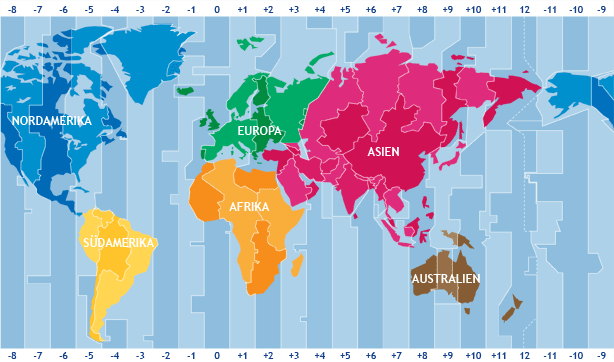
\includegraphics[scale=0.5]{zeitzonen_weltkarte.jpg}
					\caption{Zeitzonen der Erde. }

					\label{img:timezones}
				\end{center}
			\end{figure}	
			\todo{ Quelle: http://www.zeitzonen.de/images/frontend/mod\_tz\_map/zeitzonen\_weltkarte.gif} 

			Die Nutzer-Zeitzone kann in Twitter über eine Liste gewählt werden.
			\todo{Bild Auswahlliste} 
			Der Wert der Nutzer-Zeitzone stellt deshalb immer eine Zeitzone dar.
			Es ist dem Nutzer nicht möglich einen Wert einzugeben der nicht einer Zeitzone entspricht.

			Allerdings ist nicht gesichert, dass der angegegebene Wert auch der Zeitzone entspricht in der sich der Nutzer aufhält.
			Der Nutzer könnte eine bewusste Fehleingabe machen oder aber die Zeitzone nicht wählen womit der Stadardwert "'Pacific Time (US and Canada)"' gewählt wird.
			In Abbildung \ref{img:gephiTimezones} wurden Tweets anhand ihres Längen- und Breitengrades platziert.
			In der Abbildung sind Tweets aus den USA zu sehen. 
			Die Farben entsprechen den gewählten Zeitzonen.

			\begin{itemize}
			 	\item Pacific Time Blau
			 	\item Eastern Time	Rot
			 	\item Central Time Grün
			 	\item Mountain Time Pink 
			 \end{itemize} 

			 Die Zeitzonen sind durch die Farben gut zu erkennen. 
			 Lediglich die dünne besiedelte Region der Mountain Time kann nur an einige Ballungszentren erkannt werden. 
			 Grundsätzlich scheint die Angabe der Zeitzone aber korrekt zu sein.

			\todo{Bei lernen Zeitzonen Problematik mit standard einbringen} 


		\subsection{Auflösen von Doppeldeutigkeiten}

			Mit der Nutzer-Zeitzone lassen sich Doppeldeutigkeiten auflösen. 

			Besteht zu einem Nutzer-Standort eine Doppeldeutigkeit, kann nicht enstcheiden werden welches geografische Objekt zugeordnet werden soll.
			Liegen die beiden geografischen Objekte allerdings in zwei unterschiedlichen Zeitzonen und der Nutzer hat diese angegegeben kann die Doppeldeutigkeit aufgelöst werden.
			Somit kann dem Nutzer die korrelte Georeferenz zugewiesen werden.
			Vorausetzung dazu ist natürlich, dass die geografischen Objekte in zwei unterschiedlichen Zeitzonen liegen und die Nutzer-Zeitzone angegegeben ist.

	\section{Verfahren zum einlernen geografischer Indikatoren am Beispiel von Twitter} 

		Um die oben genannten Probleme beheben zu können soll ein Lernverfahren entwickelt werden.
		Dabei sollen aus einer Tweet-Sammlung die genutzten geogarfischen Indikatoren und deren Zuordnung zu einer Georeferenz automatisch gelernt werden.
		Es soll eine Georeferenz-Basis erzeugt werden, welche es ermöglicht den genutzten geografischen Indikatoren eine Georeferenz zuzuweisen. 

		Der Vorteil besteht darin, dass eine domänenspezifische Georeferenz-Basis geschaffen wird welche potenziell mehr geografische Indikatoren zuordenen kann als ein normales Ortsverzeichnis.
		Es können dadurch domänenspezifische Eigenheiten bei der Eingabe berücksichtigt werden. 
		Auch domäneninterne Begriffe sollen hierdurch gelernt werden können. 

		Zunächst soll ein genereller Ablauf zum einlernen geografischer Indikatoren vorgestellt werden.
		Danach werden die nötigen Vorverarbeitungsschritte für den Nutzer-Standort und die Nutzer-Zeitzone vorgestellt.
		Anhand desssen wird die in Abschnitt \ref{sec:generelleStruktur} vorgestellte Struktur der Georeferenz-Basis angepasst und erweitert.
		Dabei wird am grundsätzlichen Prinzip nichts geändert, es wird nach wie vor einem Referenzwert eine Georeferenz zugewiesen.
		Die Referenzwerte leiten sich dabei aus den potenziellen geografischen Indikatoren ab.

		Zum Schluss wird erläutert wie aus den gelernten Daten einem Twitter-Nutzer eine Georeferenz zugewiesen werden kann.  

		%Zu diesem Thema in einlernen. Durch das einlernen werden die in der jeweiligen Domäne verwendeten Toponyme berücksichtigt. Man ist nicht auf die Vollständigkeit einer Georeferenz-Basis und aufwändige Abfragen auf mehrere verschiedene QUellen angewiesen.
		% Spaäter in lernen: es ist natürlich klar, das die Toponyme auch genutzt werden müssen um diese einlernen zu können. Wird beispielsweise ein Spitzname einer Stadt nur von einem Nutzer verwendet wird dies nicht dazu führen diesen Ort mit dem Namen zu verknüpfen. Eine Anhäufung desselben Wertes an einem bestimmten Ort jedoch, lässt darauf schliessen, dass dieser Wert in irgendeiner Verbindung mit dem Ort steht.
		% Insbesondere gilt dies für blablablubb

		\subsection{Generelles Verfahren zum einlernen der Georeferenz-Basis}

			Um die Georeferenz-Basis einzulernen soll nun ein generelles Verfahren vorgeschlagen werden.
			Es muss mindestens ein Wert vorhanden sein aus welchem unmittelbare oder mittelbare geografische Indikatoren extrahiert werden können.
			Um den Wert für die Georeferenz zu bestimmen muss zu jedem dieser Werte eine geografische Koordinate vorhanden sein.

			Die Tweet-Sammlung beinhaltet pro Datensatz zwei Werte aus denen geografische Koordinaten extrahiert werden können.
			Jedem solchen Paar ist zusätzlich eine geografische Koordinate zugewiesen.
			Womit die Tweet-Sammlung die Anforderungen erfüllt.

			In Abbildung \ref{img:LernverfahrenAllg} ist der generelle Ablauf des Lernverfahrens am Beispiel der Twitter-Daten dargestellt.
			Es wird der Nutzer-Standort und die Nutzer-Zeitzone einer Vorverarbeitung unterzogen. 
			Daraus resultieren die geografischen Indikatoren.
			Diese wiederum werden mit der zugehörigen geografischen Koordinate in der Georeferenz-Basis gespeichert. 
			So kann jedem geografischen Indikator eine Georeferenz zugeordnet werden.

		\subsection{Vorverarbeitung des Nutzer-Standortes und der Nutzer-Zeitzone}

			Aus dem Nutzer-Standort und der Nutzer-Zeitzone werden durch die Vorverarbeitung mehrere Werte erzeugt. 
			Diese Werte müssen nicht zwangsweise einen gegrafischen Indikator darstellen. 
			Sie werden deshalb potenzielle geografische Indikatoren genannt.
			Bei unmittelbaren geografischen Indikatoren kann zunächst nicht entschieden werden ob diese einen geografischen Indikator darstellen oder nicht.
			Es ist also sinnvoll keine Werte zu verwerfen welche einen mittelbaren geografischen Indikator darstellen könnten.

			Durch die Vorverarbeitung sollen nun potenzielle geografische Indikatoren erzeugt werden.
			
			Ziel ist es aus dem Nutzer-Standort möglichst viele Informationen zu extrahieren und etwaige Probleme zu beseitigen.

			In der folgenden Liste sind einige Nutzer-Standorte angegeben. 
			Anhand dieser Liste sollen die Vorverarbeitungsschritte motiviert und demonstriert werden.

			\begin{multicols}{2}
			\begin{enumerate}
				\item Bélem-PA
				\item West Sussex, England
				\item South Florida
				\item Pitmedden,  Scotland, UK
				\item Mato Grosso \& Rio de Janeiro
				\item -****-
				\item USA \textbackslash/ Los Angeles
				\item Nottingham\textbackslash/London
				\item Los Angeles, USA
				\item I $\heartsuit$ New York 
				\item $\dagger\textasciitilde$ Los Angeles$\textasciitilde\dagger$
				\item earth-sea
				\item In front of the computer
				\item 11th Dimension | California
				\item York
				\item York
			\end{enumerate}
			\end{multicols}
				
			\subsubsection{Eliminierung von Sonder- und Satzzeichen} 

				Es fällt auf, dass oft Sonder- und Satzzeichen verwendet werden. 
				Beispielsweise als Trenner zwischen Toponymen unterschiedlicher geografischer Hierarchieebenen wie bei "'West Sussex, England"', "'USA \textbackslash/ Los Angeles"' oder "'Bélem-PA"'.
				Das Trennzeichen wird nicht einheitlich verwendet.  
				Es kann deshalb nicht entschieden werden ob ein Satzzeichen als Trenner zweier Hierarchiebenen fungiert oder nicht.
				Bei "'USA \textbackslash/ Los Angeles"' wird \textbackslash/ als Trenner für Hierarchieebenen verwendet bei "'Nottingham\textbackslash/London"' werden zwei Städte angegeben.
				Es ist also insbesondere nicht klar welcher Zusammenhang zwischen den Toponymen, die durch ein Zeichen getrennt sind, besteht. 

				Bei "'I $\heartsuit$ New York "' werden Sonderzeichen zum ausdrücken von Emotionen genutzt.
				In "'$\dagger\textasciitilde$ Los Angeles$\textasciitilde\dagger$"' werden Sonderzeichen als Dekoration genutzt.
				Einige Nutzer-Standorte bestehen ausschließlich aus Sonder- und Satzzeichen.

				Zur Ableitung eines geografsichen Bezugs bringen die Sonder- und Stazzeichen keinen Mehrwert.
				Es gibt Fälle in denen Sonder- oder Satzzeichen Bestandteil des Toponyms sein.
				Ein Beispiel hierfür wäre "'3. Arrondisement"' in Paris, das weglassen des Punktes würde hier aber zu keinen Problemen führen.
				
				Grundsätzlich ist es aufgrund der Vielfalt schwierig definitiv zu entscheiden ob Satz- und Sonderzeichen einen Mehrwert bieten bei der Georeferenzierung. 
				Das hinzufügen von Satz- und Sonderzeichen kann allerdings mehr Probleme mit sich bringen als es Vorteile bringt.
				Es sollen deshalb in einem ersten Vorverarbeitungsschritt alle Sonder- und Satzzeichen entfernt werden. 

				Liste nach dem entfernen von Sonder- und Satzzeichen:

				\begin{multicols}{2}
					\begin{enumerate}
						\item Bélem PA
						\item West Sussex England
						\item South Florida
						\item Pitmedden Scotland UK
						\item Mato Grosso Rio de Janeiro
						\item 
						\item USA Los Angeles
						\item Nottingham London
						\item Los Angeles USA
						\item I New York 
						\item Los Angeles
						\item earth sea
						\item In front of the computer
						\item 11th Dimension California
						\item York
						\item York
					\end{enumerate}
				\end{multicols}

				Der Wert 6 existiert nun nicht mehr, der Wert ist leer und wird somit nicht weiter betrachtet.

				Der Vorteil besteht darin, dass unnötige Sonder- und Satzzeichen entfernt werden und mögliche geografische Indikatoren einfacher verarbeitet werden können.

			\subsubsection{Zusammenfassen von Toponymen}

				In diesem Schritt sollen Toponyme, welche aus zwei oder mehr Wörtern bestehen mit Hilfe eines Ortsverzeichnisses zusammengefasst werden. 
				Dies kann nur für bekannte Toponyme durchgeführt werden.
				Damit bilden beispielsweise "'Los"' und "'Angeles"' eine Einheit. 
				Dies soll mit einem + Zeichen gekennzeichnet werden.

				Daraus resultiert:

				\begin{multicols}{2}
					\begin{enumerate}
						\item Bélem PA
						\item West+Sussex England
						\item South Florida
						\item Pitmedden Scotland UK
						\item Mato+Grosso Rio+de+Janeiro
						\item USA Los+Angeles
						\item Nottingham London
						\item Los+Angeles USA
						\item I New+York 
						\item Los+Angeles
						\item earth sea
						\item In front of the computer
						\item 11th Dimension California
						\item York
						\item York
					\end{enumerate}
				\end{multicols}
				In diesem Schritt wird insbesondere keine Georeferenzierung vorgenommen. 
				Dieser Schritt dient dazu, möglichst früh vorhandenes Wissen über Toponyme einzubeziehen.

				Im wesentlichen sollen die Werte hiermit für die nächsten Verarbeitungsschritte vorbereitet werden.

			\subsubsection{Alphanumerische Sortierung}

				In diesem Schritt sollen die Werte alphanumerisch sortiert werden. 
				Dadurch ist die Reihenfolge in der die Werte angegeben werden unerheblich.

				Nach der Sortierung liegt folgende Tabelle vor:

				\begin{multicols}{2}
					\begin{enumerate}
						\item Bélem PA
						\item England West+Sussex
						\item Florida South
						\item Pitmedden Scotland UK
						\item Mato+Grosso Rio+de+Janeiro
						\item Los+Angeles USA
						\item London Nottingham
						\item Los+Angeles USA
						\item I New+York 
						\item Los+Angeles
						\item earth sea
						\item computer front In of the 
						\item 11th California Dimension 
						\item York
						\item York
					\end{enumerate}
				\end{multicols}

				Die Werte 6 und 8 sind nun gleich. 
				Durch die Sortierung werden Werte mit gleichem Inhalt aber unterschiedlicher Reihenfolge angeglichen.
				Durch das zusammenfassen der Toponyme im vorherigen Schritt werden bekannte Toponyme nicht getrennt.
				Es wird eine unnötige Fragmentierung der Werte vermieden.

				Dieser Schritt stellt aber einen Kompromiss dar.
				Es werden zwar Werte mit gleichem Inhalt und unterschiedlicher Reihenfolge angeglichen.
				Aber es werden auch potenzielle Toponyme, die aus mehreren Werten bestehen, auseinandergezogen.
				Aus "'Motor City Michigan USA"' würde "'City Michigan Motor USA"' entstehen.
				Der Zusammenhang zwischen Motor und City wäre nicht mehr vorhanden.  

			\subsubsection{Erzeugung von N-Grammen}

				Es sollen nun N-Gramme bis zum Grad 3 erzeugt werden. 
				Aus einem Nutzer-Standort werden mehrere potenzielle geografische Indikatoren erzeugt.
				Dieses Vorgehen löst gleich mehrere Probleme.

				Zum ersten können sowohl geografische Indikatoren als auch Werte die kein geografischen Indikator darstellen in den Nutzer-Standorten vorhanden.
				Durch die Erzeugung von N-Grammen können diese getrennt voneinander betrachtet werden.
				Es löst das Problem des partiellen geografischen Bezugs des Nutzer-Standortes aus \ref{subsec:partiellerGeografischerBezug} in der Hinsicht, dass die Werte für die weitere Verarbeitung getrennt betrachtet werden können.

				Zum zweiten können in einem Nutzer-Standort mehrere geografische Indikatoren enthalten sein.  
				Der Wert "'Pitmedden Scotland UK"' enthält mit "'UK"' das Land, mit "'Scottland"' den Landesteil und mit "'Pitemedden"' eine Stadt. 
				Mit der Georeferenz aus dem zugehörigen Tweet kann nun allen drei Werten eine Georeferenz zugeordnet werden.

				Aber auch zwei verschiedene Städte wie "'Nottingham\textbackslash/London"' können in einem Wert vorkommen.
				Diese werden zu "'Nottingham\textbackslash/London"', "'Nottingham"' und "'London"'.
				Wird hier wiederum beiden Werten die geografische Koordinate zugeordnet können drei Fälle auftreten.
				Erstens: Der Nutzer war in keiner der beiden Städte als er den Tweet abgesetzt hat. 
				Damit sind beide Zuordnungen unbrauchbar.
				Zweitens: Er war in einer der beiden Städte, dann ist zumindest einer der entstandenen Datensätze brauchbar.
				Dies löst das Problem aus \ref{subsec:wiederspruechlicheBezuege} in der Hinsicht, dass die Werte für die weitere Verarbeitung getrennt betrachtet werden können.

				Besteht allerdings eine Beziehung der Werte zueinander, kann diese durch Bi- und Trigramme abgebildet werden.
				Aus "'Pitmedden Scotland UK"' wird "'Pitmedden Scotland"', "'Scotland UK"' und "'Pitmedden Scotland UK"' erzeugt.

				Dieser Schritt soll nur an einigen ausgewählten Beispielen aus der Liste erfolgen die Bestandteile der N-Gramme werden mit \textless \textgreater gekennzeichnet:

				\begin{multicols}{2}
					\begin{enumerate}
						\item \textless England\textgreater   \textless West+Sussex\textgreater  
						\item \textless England\textgreater  
						\item \textless West+Sussex\textgreater  
						\item \textless Mato+Grosso\textgreater   \textless Rio+de+Janeiro\textgreater  
						\item \textless Rio+de+Janeiro\textgreater  
						\item \textless Mato+Grosso\textgreater  
						\item \textless 11th\textgreater   \textless California\textgreater   \textless Dimension\textgreater   
						\item \textless 11th\textgreater   \textless California\textgreater  
						\item \textless California\textgreater   \textless Dimension\textgreater   
						\item \textless 11th\textgreater  
						\item \textless California\textgreater  
						\item \textless Dimension\textgreater   
						\item \textless York\textgreater  
						\item \textless York\textgreater  
					\end{enumerate}
				\end{multicols}
				 Der Wert 7 ist ein Trigramm.
				 Bei den Werten 1,4,8 und 9 handelt es sich um Bigramme. 
				 Die Werte von 2,3,5,6,10,11 und 12 sind Unigramme.

				Auch hier entsteht aufgrund des zusammenfassens bekannter Toponyme keine Fragmentierung der Werte, da zusammengehörige Toponyme gemeinsam betrachtet werden.

			\subsubsection{Hinzufügen der Zeitzone}

				Es soll an dieser Stelle die Zeitzone hinzugefügt werden.
				Da die Zeitzone eine begrenzte Anzahl an Werten darstellt und diese vom Nutzer nicht frei eingegeben werden können muss hier keine weitere Vorverarbeitung vorgenommen werden.

				Jeder Wert der in der aktuellen Liste vorkommt soll einmal mit und einmal ohne Zeitzone existieren. 
				Damit wird garantiert, das eingelrnete Werte die eine falsche Zeitzone aufweisen trotzdem berücksichtigt werden bei einer Anfrage. 

				Auch hier wird die Liste weiter eingeschränkt und es werden lediglich noch zwei Beispiele betrachtet.
				\begin{multicols}{2}
					\begin{enumerate}
						\item England West+Sussex
						\item \textless England\textgreater  
						\item \textless West+Sussex\textgreater  
						\item \textless England\textgreater   \textless West+Sussex\textgreater   London
						\item \textless England\textgreater   London
						\item \textless West+Sussex\textgreater   London
						\item \textless 11th\textgreater   \textless California\textgreater   \textless Dimension\textgreater    
						\item \textless 11th\textgreater   \textless California\textgreater  
						\item \textless California\textgreater   \textless Dimension\textgreater   
						\item \textless 11th\textgreater  
						\item \textless California\textgreater  
						\item \textless Dimension\textgreater   
						\item \textless 11th\textgreater \textless California\textgreater   \textless Dimension\textgreater   Pacific Time (US \& Canada)
						\item \textless 11th\textgreater   \textless California\textgreater   Pacific Time (US \& Canada)
						\item \textless California\textgreater   \textless Dimension\textgreater   Pacific Time (US \& Canada)
						\item \textless 11th\textgreater   Pacific Time (US \& Canada)
						\item \textless California\textgreater   Pacific Time (US \& Canada)
						\item \textless Dimension\textgreater   Pacific Time (US \& Canada)
						\item York
						\item \textless York\textgreater   London
						\item York
						\item \textless York\textgreater   Eastern Time
					\end{enumerate}	
				\end{multicols}
				Mit Hilfe der Zeitzone können nun auch die beiden letzten Einträge unterschieden werden. 
				Zum einen York in England zum anderen York in den USA. 
				Dies löst das Problem der Mehrdeutgkeiten von Toponymen. 
				Mit Hilfe der zusätzlichen Zeitzone können geografische Objekte, zumindest wenn sie in zwei verschiedenen Zeitzonen liegen, unterschieden werden.

			\subsubsection{Fazit} 

				Nach der Vorverarbeitung liegen eine Menge von potenziellen geografischen Indikatoren mit zugehörigen geografischen Koordinaten vor.
				Bei der Vorverarbeitung wurden einige Probleme des Nutzer-Standortes und bei der Verwendung von Toponymen beseitigt.

				Diese durch die Vorverarbeitung erzeugten potenziellen geografischen Indikatoren können nun in der Georeferenz-Basis gespeichert werden.
				Mit der so erzeugten Georeferenz-Basis ist es grundsätzlich möglich eine Georeferenzierung durchzuführen. 
				Allerings wird jedem potenziellen geografischen Indikator eine Georeferenz zugeordnet.
				Das ist grundsätzlich problematisch, da Indikatoren die keinen geografischen Bezug aufweisen eine Georeferenz zugeordnet wird. 
				Dies kann bei der Georeferenzierung zu Fehlern führen.
				Es sollte entschieden werden können ob es sich um einen geografischen Indikator handelt oder nicht. 

				Des weiteren können zu einem Referenzwert beliebig viele Datensätze existieren, selbst wenn diese auf denselben Ort verweisen. 
				Bei einer Abfrage an die Datenbank werden potenziell große Mengen an Datensätzen zurückgeliefert die alle auf dieselbe Georeferenz verweisen.

		\subsection{Häufigkeistwert}

			Es soll nun ein Häufigkeitswert in der Georeferenz-Basis eingeführt werden.
			Der Häufigkeitswert soll angeben wie oft eine Kombination aus Referenzwert und Georeferenz in der Georeferenz-Basis vorhanden ist.
			Dadurch werden Duplikate in der Georeferenz-Basis vermieden.
			Zusätzlich kann ermittelt werden ob ein Referenzwert an einer bestimmten Position gehäuft auftritt.

			Beim abspeichern eines neuen Datensatzes soll nun zunächst geprüft werden ob dieser bereits in der Georeferenz-Basis vorhanden ist. 
			Ist dies der Fall, so wird der Häufigkeitswert des entsprechenden Eintrags um 1 erhöht.
			Ist der Datensatz noch nicht gespeichert so wird ein neuer Datnesatz angelegt und der Häufigkeitswert mit 1 initialisiert.

			Der Häufigkeitswert misst damit wie oft ein potenzieller geografischer Indikator an einer geografischen Position vorkommt.
			Es ist zu erwarten, dass ein Indikatoren mit geografischem Bezug gehäuft an einer bestimmten geografischen Position oder Region auftritt.
			Während Indikatoren die keinen geografischen Bezug haben sehr verteilt oder nur sehr selten auftreten. 

			Die Georeferenz besteht aus den geografischen Koordinaten des zugehörigen Tweets.
			Die geografische Position wird zumeist mit Hilfe von GPS-Modulen mobiler Endgeräte wie Smartphones bestimmt. 
			Diese können eine Position oft auf wenige Meter genau bestimmen.
			Das bedeutet, zwei Tweets die wenige Meter voneinander abgesetzt wurden haben unterschiedliche Werte für den Längen- und Breitengrad.
			Dies kann für die Bestimmung der Häufigkeiten problematisch sein, da die Werte in der Regel nicht exakt übereinstimmen.
			Um dies zu umgehen sollen die geografischen Koodinaten auf Städte abgebildet werden.
			Dazu müssen die geografischen Koordinaten einer Vorverarbeitung unterzogen werden.

		\subsection{Vorverarbeitung der geografischen Koordinaten}

			Die geografischen Koordinaten sollen auf Stödte aufgelöst werden.
			Dies enstpricht der untersten Ebene der geografischen Hierarchie.
			Insbesondere werden damit auch alle anderen geografischen Hierarchieebenen bestimmt.

			Jeder geografischen Koordinate soll die am nächsten gelegene Stadt zugeordnet werden.
			Als Ergebnis liegt nun pro Referenzwert statt einer geografischen Koordinate eine Stadt vor.
			Dies kann als Übergang einer kontinuierlichen Darstellung durch geografische Koordinaten zu einer diskreten Darstellung durch Städte angesehen werden. 
			
			Durch die Nearest-Neighbour Zuordnung der geografischen Koordinaten zu Städten wird der Globus in Voronoi-Regionen eingeteilt.
			Die Punkte zur Erzeugung der Voronoi-Regionen bilden dabei die Städte. 
			Jeder Voronoi-Region kann also eine Stadt zugewiesen werden.
			Wird ein Tweet innerhalb einer Voronoi-Region abgesetzt wird er der enstprechenden Stadt zugeordnet.

			In Abbildung \ref{img:nearestNeighbour} ist die Zuordnung schematisch dargestellt.

			\todo{nearestNeighbourImage} 

		\subsection{Finale Struktur der Georeferenz-Basis} \label{subsec:finaleStruktur} 

			Hier soll nun die Finale Struktur der Georeferenz-Basis vorgestellt werden.
			Mit dem Häufigkeitswert ist ein neuer Wert pro Datensatz hinzugekommen.
			Des weiteren wurde die Georeferenz auf eine Stadt aufgelöst und damit implizit die Administrationsebene erster Ordnung (Adm1), die Adminstrationsebene zweiter Ordnung (Adm2) und das Land. 
			Neben der Stadt sollen auch die anderen Ebenen pro Datensatz hinterlegt sein.
			Die daraus resultiernde Struktur der Georeferenz-Basis ist in \ref{tab:strukturMitHierarchie1} inklusive einiger Beispieleinträge dargestellt.

			\begin{table}[htpb]
				\caption{Struktur der Georeferenz-Basis mit geografischer Hierarchie} 
				\centering
				\begin{tabular}{|c|c|c|c|c|c}
					\hline
					Referenzwert & Stadt & Adm2 & Adm1 & Land & Häufigkeit \\
					\hline\hline
					\textless Los+Angeles\textgreater   \textless USA\textgreater   & Los Angeles & Los Angeles County & California & United States of America & 30 \\
					\hline
					\textless Los+Angeles\textgreater   \textless USA\textgreater   & San Francisco & San Francisco County & California & United States of America & 3 \\
					\hline
					\textless Los+Angeles\textgreater   & Los Angeles & Los Angeles County & California & United States of America & 70\\
					\hline
					\textless USA\textgreater   & Los Angeles & Los Angeles County & California & United States of America & 80 \\
					\hline
					\textless Heilbronn\textgreater   & Heilbronn & Regierungsbezik Stuttgart & Baden-Württemberg & Bundesrepublik Deutschland & 90\\
					\hline
				\end{tabular}
				\label{tab:strukturMitHierarchie1} 
			\end{table} 

			Eine andere Darstellung für die Georeferenz-Basis kann in \ref{img:hierarchieUndReferenz} betrachtet werden.
			Der Baum stellt die geografische Hierarchie dar, an die Blätter wird der Referenzwert und die zugehörige Häufigkeit angehängt.

			\todo{Hierarchiebaum mit Referenzwerten}  

		\subsection{Verfahren zum einlernen der Georeferenz-Basis}

			Hier soll nun ein Überblick über das gesamte Verfahren zum einlernen der Georeferenz-Basis gegeben werden.
		
			Zunächst werden die einzelnen Vorverarbeitungsschritte für den Nutzer-Standort und die Nutzer-Zeitzone durchgeführt.
			Parallel kann der Längen- und Breitengrad aufgelöst werden.
			Die dadurch entstandenen potenziellen geografischen Indikatoren und die zugehörige Georeferenz wird nun in die Georeferenz-Basis gespeichert. 
			Dabei wird überprüft ob dieser Datensatz bereits vorhanden ist. 
			Ist dies der Fall, wird der Häufigkeistwert des entsprechenden Datensatzes inkrementiert.
			Ist der Datensatz noch nicht vorhanden wird er angelegt und der Häufigkeitswert mit 1 initialisiert.

			Die Vorverarbeitung extrahiert dabei zusätzliche Informationen aus dem Nutzer-Standort.
			Durch die Bereiningung der Werte im Nutzer-Stadort, die alphanumerische Sortierung, das identifzieren von Toponymen mit mehreren Worten und die darauffoglende Erzeugung von N-Grammen werden zusätzliche Infomrationen aus jedem Nutzer-Standort gewonnen.
			Die Nutzer-Zeitzone wird einbezogen um Doppeldeutigkeiten auflösen zu können.

			Durch die neue Datenstruktur, mit dem Häufigkeitswert und der abgebildeten geografischen Hierarchie, lassen sich nun tiefergehende Analysen durchführen um eine robuste Georeferenzierung zu ermöglichen. 
			Der Häufigkeitswert gibt dabei an wie oft ein Referenzwert in der Nähe einer Stadt vorkommt.

			Durch dieses Verfahren lässt sich eine Datenbasis erzeugen die domänenspezifische Eigenheiten, in Bezug auf die Verwendung spezieller Begriffe oder Formulierungen, berücksichtigt.
			Des weiteren werden Toponyme, die in Ortsverzeichnissen unter Umständen nicht hinterlegt sind, berücksichtigt.
			Auch mittelbare geografische Indikatoren, zum Beispiel die Verwendung spezieller Begriffe in einer geografischen Region, können einbezogen werden.

			Die so entstandene Georeferenz-Basis kann nun zur Georeferenzierung verwendet werden. 

	\section{Verfahren zu Georeferenzierung am Beispiel von Twitter}

		Es soll nun das Verfahren zu Georeferenzierung am Beispiel von Twitter vorgestellt werden.
		Die Georeferenz-Basis aus Unterkapitel \ref{subsec:finaleStruktur} dient dabei als Grundlage zur Ermittlung einer Georeferenz.

		Einem Twitter-Nutzer, dessen geografische Position nicht bekannt ist, soll automatisch eine Georeferenz zugewiesen werden.
		Die Georeferenz soll dabei einer der Ebenen der geografischen Hierarchie aus Abschnitt \ref{chp:Grundlagen} entsprechen. 
		Wie beim einlernen der Georeferenz-Basis werden aus dem Nutzer-Standort und der Nutzer-Zeitzone zunächst potenzielle geografische Indikatoren erzeugt.
		Diese Indikatoren werden in der Georeferenz-Basis nachgeschlagen.
		Durch die Vorverarbeitung können mehrere potenzielle geografische Indikatoren entstehen. 
		Zudem können zu jedem potenziellen geografischen Indikator mehrere Einträge in der Georeferenz-Basis vorhanden sein.
		Bei einer Abfrage auf die Georeferenz-Basis ensteht somit eine Menge von Datensätzen.
		Um eine Georeferenz zuweisen zu können müssen diese Datensätze ausgewertet werden.
		
		Im folgenden soll zunächst gezeigt werden wie mit Hilfe des Häufigkeitswertes geografische Indikatoren identifiziert werden können.
		Danach sollen wiederum mit Hilfe des Häufigkeitswertes die Konfidenzen berechnet werden. 
		Zum Schluss osll gezeigt werden wie unter Einbeziehung der geografischen Hierarchie die Georeferenzierung weiter verebessert werden kann.  
		Es soll deshalb zunächst darauf eingegangen werden, wie mit Hilfe des Häufigkeitswertes allein 

		\subsection{Identfizierung eines geografischen Indikators}
			
			Grundsätzlich ist die Frage zu beantworten: Wie kann ein geografischer Indikator identifiziert werden?
			Die Frage kann auch anders gestellt werden: Wie kann vermieden werden, dass einem Indikator ohne geografischen Bezug eine Georeferenz zugewiesen wird?
			Dies ist wichtig, denn durch eine solche Zuweisung kann es zu Fehlern in der Georeferenzierung kommen.
			Dies wiederum führt zu schlechten und unzuverlässigen Ergebnissen.	
			Die Identfizierung geografischer Indikatoren beinhaltet insbesondere die Identifizierung mittelbarer und unmittelbarer geografischer Indikatoren. 
			Es wird nicht unterschieden ob es sich um einen mittelbaren oder unmittelbaren Indikator handelt, lediglich der geografische Bezug des Indikators soll vorhanden sein.

			Die Zuordnung einer Georeferenz zu einem Indikator erfolgt grundsätzlich über die Referenzwerte in der Georeferenz-Basis.
			Anhand dieser soll entschieden werden ob der Indikator geografischen Bezug hat oder nicht.
			Das bedeutet mit einer Analyse, der aus einer Abfrage des Indikators resultierenden Datensätze, soll entschieden werden ob es sich um einen geografischen Indikator handelt.  
			Das Problem kann damit auf die Referenzwerte der Georeferenz-Basis projiziert werden.

			Anhand des Häufigkeitswertes zu einem Referenzwert kann entschieden werden, ob es sich um einen geografischen Indikator handelt oder nicht.
			Der Häufigkeitswert gibt an wie oft ein Referenzwert in einer bestimmten Region, zunächst die Voronoi-Region der entsprechenden Stadt, vorkommt.			 
			
			Es ist zu erwarten, dass in der Nähe einer Stadt der Stadtname im Nutzer-Standort häufiger vorkommt als in der Nähe einer anderen Stadt.
			In Abbildung \ref{img:ULNewYork} sind die vorkommen von "'New York"' im Nutzer-Stadort und den zugehörigen Positionen, von welchen der Tweet abgesetzt wurde aufgetragen.
			Dabei wurde nur nach dem Teilstring "'New York"' im Nutzer-Stadort gesucht und keine weitere Verarbeitung vorgenommen.
			Es ist deutlich eine Häufung um die Stadt und den Bundesstaat New York zu erkennen. 
			Allgemein werden Referenzwerte mit einem geografischen Bezug in der Region, auf die sie Bezug nehmen, öfter vorkommen als anderswo.



				Referenzwerte ohne geografischen Bezug





			Es muss also die Frage beantwortet werden ob und vor allem wie geografische Indikatoren identifiziert werden können. 



			Mit anderen Worten, handelt es sich bei einem gegebenen Indikator um einen geografischen Indikator oder nicht.
			Ein geografischer Indikator weißt grundsätzlich einen geografischen Bezug auf. 

			Dies kann mit Hilfe der Georeferenz-Basis geprüft werden.
			Bei einer Abfrage eines potenziellen geografischen Indikators auf die Georeferenz-Basis erhält man eine Menge an Datensätzen welche den Referenzwert, den Häufigkeitswert und eine Georeferenz beinhalten.

			Um zu entscheiden, ob ein potenzieller geografischer Indikator einen geografischen Bezug hat, kann nun einfach der Häufigkeitswert betrachtet werden.
			Denn dieser gibt an wie häufig ein Referenzwert innerhalb einer geografischen Region aufgetaucht ist. 
			Die geografische Region ist dabei die  


			Diese Frage kann mit Hilfe der Häufigkeitswerte beantwortet werden.
			Es ist zu erwarten, dass ein Refrenzwert mit geografischem Bezug in derjenigen geografischen Region zu der der geografische Bezug gehört öfter auftauch als anderswo.


			Es ist insbesondere zu beachten, dass Referenzwerte ohne geografischen Bezug sehr verteilt oder nur sehr selten vorkommen. 

			\todo{Bild the für verteilt und Beispiel für sehr selten} 

			Der Häufigkeitswert gibt an wie oft ein  


			\todo{Images ULNewYork ULThe}

		\subsection{Berechnung der Konfidenz} 

		\subsection{Einbeziehung der geografischen Hierarchiebene} 









		\subsection{Berechnung von Konfidenzen}

			Die Konfidenz setzt sich aus zwei Werten zusammen. 
			Zum einen gibt der Häufigkeitswert

			Die Konfidenzen lassen sich einfach über die Häufigkeitswerte berechnen. 
			Dabei wird die Rückgabe aus der Georeferenz-Basis eingeteilt in die Ordnung der N-Gramme. 
			Das bedeutet es werden Uni-, Bi- und Trigramme getrennt voneinander betrachtet.
			Aus den zurückgegebenen Datensätzen entstehen so 3 Gruppen.

			Innerhalb jeder Gruppe werden nun die 

			Mit Hilfe der Häufigkeitswerte kann nun für die einzelnen Datensätze der Anteil berechnet werden. 
			Dieser Anteil stellt die Konfidenz dar. 

			Wie bereits erwähnt kann die Datenbasis auch als Hierarchiebaum dargestellt werden. 
			Die erste fünf Ebenen bilden die geografische Hierarchie ab. 
			Die Blätte des Baumes beinhalten den Referenzwert und den zugehörigen Häufigkeitswert.


		Dies soll an einem Beispiel erläutert werden.

		Der Nutzer-Standort beinhaltet den Wert "'Love Karlsruhe, Deutschland "' dieser wird in folgende potenzielle Indikatoren zerlegt.

		\begin{multicols}{2}
			\begin{enumerate}
			   		\item Love
			   		\item Karlsruhe
			   		\item Deutschland
			   		\item Love Karlsruhe
			   		\item Karlsruhe Deutschland
			   		\item Love Karlsruhe Deutschland
			\end{enumerate}   	
		\end{multicols}

		Zu jedem dieser Indikatoren können mehrere Einträge in der Datenbasis vorhanden sein. 
		Vor allem "'Love"' wird mehrere Einträge haben, da kein geografischer Bezug besteht und dieser Wert global auftritt.
		Auch für Deutschland werden einige Einträge vorhanden sein "'"'    
		
		


		Die daraus resultiernden Datensätze enthalten alle Informationen, die zu diesen Werten verfügbar sind.
		Durch eine Analyse dieser Datensätze kann nun dem Nutzer eine Georeferenz zugewiesen werden.
		Die Analyse soll einige der oben genannten Probleme bei der Verwendung des Nutzer-Standortes

		In Abbildung \ref{img:GeorefTable} ist der Ablauf an einem Beispiel schematisch dargestellt.  

		Es soll nun gezeigt werden wie mit Hilfe der Georeferenz-Basis und der erarbeiteten Struktur eine Georeferenzierung durchgeführt werden kann.

		Es soll zunächst ein Verfahren zur Berechnung von Konfidenzen basierend auf den Häufigkeitswerten erarbeitet werden. 
		Danach werden die noch bestehenden Probleme aufgelistet und es wird erläutert wie sich diese durch die Berechnung der Konfidenz lösen lassen. 

		Danach wird erklärt wie die geografische Hierarchie genutzt werden kann um die Georeferenzierung zu verbessern.


		Bei der Georeferenzierung soll einem Twitter-Nutzer, dessen geografische Position unbekannt ist, eine Georeferenz zugewiesen werden.
		Dabei soll dessen Nutzer-Standort und die Nutzer-Zeitzone als Indikatoren dienen. 
		Diese werden zunächst derselben Vorverearbeitung unterzogen wie beim einlernen der Georeferenz-Basis.
		Dadurch werden zusätzliche Informationen extrahiert.


		Die Probleme aus bei der Verwendung des Nutzer-Standortes und den darin enthaltenen Toponymen können durch eine Analyse der Datenbassi 



\todo{Als Beispiel bei Analyse: Drittens: Die beiden Städte liegen im gleichen Land. 
				Dann ist zumindest das Land, welches aus der Stadt ermittelt werden kann und man hat noch eine zusätzliche Information für die Landesebene gewonnen}  
				 sind entweder beide Werte nicht korrekt, wenn der Nutzer sich nicht in einer der Städte aufgehalten hat




		\section{Identifizierung geografischer Indikatoren}

			Die Frage ob es sich bei dem Referenzwert tatsächlich um einen geografischen Indikator handelt kann mit Häufigkeitswerten beantwortet werden.
			Kommt in einer Voronoi-Region einer Stadt besonders häufig ein bestimmter Referenzwert vor ist dieser sehr wahrscheinlich ein gegografischer Indikator.

			Handelt es sich nicht um einen geografischen Indikator wird der Wert entweder sehr verteilt oder sehr selten vorkommen.
			Im ersten Fall existieren zwar viele Einträge in der Datenbank, aber der Häufigkeitswert wird sehr niedrig sein.
			Im zweiten Fall wird lediglich der Häufigkeitswert sehr gering sein.




		
				
			\subsubsection{Fazit} 

				Der Referenzwert muss nun nicht zusätzlich auf ein geografisches Objekt der gewünschten Hierarchieebene aufgelöst werden.
				Aus der Georeferenz-Basis kann der Referenzwert für alle Hierarcheieebenen direkt bestimmt werden.

				NAch wie vor ist nicht bekannt was für ein geografisches Objekt der Referenzwert beschreibt, ist der Referenzwert ein Land wird 



		
			\paragraph{Hierarchiebenen}   


			Soll nun ein gegrafischer Indikator



			Dadurch wird zunächst das Problem gelöst, dass meherere Einträge zu einem Referenzwert existieren.
			Denn diese werden nun, vorausgesetzt die Georeferenz stimmt überein 






			





	\section{Einlernen einer Georeferenz-Basis}

			Das Problem besteht grundsätzlich darin, dass nicht alle verwendeten Toponyme bekannt sein können. 
			Zum anderen ist nicht bekannt welche Werte einen mittelbaren geografischen Indikator darstellen.




			Die oben genannten Datenbasen  

				Hinzu soll das Wort Guatsle und Filzl kommen.
				Beide Wörter beschreiben keine Kartoffel, haben aber aufgrund des Dialekts einen 
				Ein Guatsle ist ein BonBon oder eine Süßigkeit und wird im württembergischen verwendet.
				Filzl bedeutet Mett und wird in der Pfalz verwendet.

				Damit sieht die Liste folgendermaßen aus.

				\begin{table}[htpb]
					\caption{verschiedene dialektische Begriffe} 
					\centering
					\begin{tabular}{|c|c|}
						\hline
						Referenzwert & Georeferenz \\
						\hline\hline
						Äbbiera & Württemberg \\
						\hline
						Guatsle & Württemberg \\
						\hline
						Grumbeer & Württemberg \\
						\hline
						Grumbeer & Pfalz \\
						\hline
						Filzl & Pfalz \\
						\hline
						Tüfte & Norddeutschland \\
						\hline
					\end{tabular}
					\label{tab:dialektZwei} 
				\end{table} 

				Mit dieser Liste ergeben sich nun einige Möglichkeiten zur Georeferenzierung.

			

			\paragraph{Beispiel für Lernen} 

				Es liegen drei Briefe vor deren Absender unbekannt ist.
				In den Briefen beschreiben die Autoren ihr Mittagessen. 
				Mit Hilfe der Georeferenz-Basis aus \ref{tab:dialektZwei} soll nun entschieden werden woher die 
				Alle Briefe sind in deutscher Sprache verfasst, es soll genügen eine geografische Region innerhalb Deutschlands zu bestimmen. \footnote{Die restlichen deutschssprachigen Länder sollen ignoriert werden}  

				Die Aufgabe besteht also darin dem Brief eine Georeferenz zuzuordnen. 
				Dies kann durch eine Analyse seines Inhaltes realisiert werden. 
				Der Inhalt eines Briefes sind in der Regel Wörter. 
				Womit jedes Wort einen potenziellen Indikator darstellt.

				Nach einer Analyse der Wörter fallen folgende drei Begriffe auf:

				

				Hat man eine solche Georeferenz-Basis erstellt können die Briefe automatisch untersucht werden.
				Für jedes Wort in den Briefen wird geprüft ob es sich um einen dieser Referenzwerte handelt. 
				Wenn ein Treffer vorliegt wird dem Brief die enstprechende Georeferenz zugewiesen.

				In diesem Beispiel werden mehrere Probleme der Georeferenzierung klar. 

				Anhand von Indikatoren wird einem übergeordneten Objekt eine Georeferenz zugewiesen. 
				Die Indikatoren können der Inhalt des Objekts sein oder diese sind auf irgendeine Art mit dem Objekt verknüpft.
				Im Beispiel eines Briefes sind die Worte im Brief potenzielle Indikatoren.



				Auch ist nicht garantiert, dass in einem Brief das Wort Kartoffel in dialektischer From vorkommt.
				In einem Geschäftsbrief werden dialektische Worte nicht vorkommen und diesen kann somit keine Georeferenz zugewiesen werden.


				Die Zuordnung ist hier mit einer Gewissen Unsicherheit verbunden. 
				Der Autor könnte unter Umständen in der Region aufgewachsen sein aber nun in einer anderen Region wohnen und dieses Wort aus Gewohnheit benutzen.
				Dies soll hier aber zunächst ignoriert werden. 


		
		
		Es gibt dabei allerdings zwei grundsätzliche Probleme.
		Zunächst muss bekannt sein, dass die Referenzwerte auch in den untersuchten Indikatoren vorkommen.
		In einem Geschäftsbrief werden keine dialektischen Begriffe genutzt werden und somit bringt die


		\begin{enumerate}
			\item Wie kann einem solchen Wert eine Georeferenz zugeordnet werden?
			\item Wie kann sichergestellt werden, dass dieser Wert auch genutzt wird und somit eine Georeferenzierung erst möglich wird?
		\end{enumerate}




			\paragraph{Zu jeder Zeichenkette ist eine Georeferenz bekannt}

				Im Beispiel in \ref{tab:simpleStruktur} ist für jedes mögliche Toponym eine Georeferenz in Form einer Adresse bekannt.
				Dadurch wird angenommen, dass alle Anfragen an die Georeferenz-Basis ausschliesslich die drei angegbenen Werte beinhalten. 
				Dabei ist nicht die Anzahl der möglichen Werte das Problem.
				Die Tabelle könnte nach beliebig erweitert werden.
				Das Problem sind Anfragen die nicht in der Georeferenz-Basis gespeichert sind.

				Es gibt mehrere Möglichkeiten wieso die Werte nicht in der Georeferenz-Basis vorhanden sind. 

				\begin{enumerate}
				 	\item Die  
				 \end{enumerate} 



			\paragraph{Die geografischen Indikatoren sind Toponyme}

				Dies muss nicht unbedingt der Fall sein. 
				Vorstellbar ist hier 

			Diese Struktur erfüllt grundsätzlich alle Eigenschaften die benötigt werden um eine Georeferenzierung durchzuführen. 
			In der Praxis ist eine Georeferenzierung auf diese Weise allerdings nur schwer umzusetzen.

			\subsubsection{Vollständigkeit der Georeferenz-Basis} 

				Im Minimalbeispiel in \ref{tab:simpleStruktur} wird davon ausgegangen, dass alle Toponyme und die zugehörigen Georeferenzen bekannt sind.		

			\subsubsection{Doppel- und Mehrdeutigkeiten bei geografischen Indikatoren} 



			\subsubsection{Einheit der Georeferenz} 


			Im obigen Beispiel werden lediglich drei Werte angegeben für die eine Georeferenz 

			\subsubsection{Erstellung einer Georeferenz-Basis zur Georeferenzierung}

				Wie kann eine solche Georeferenz-Basis nun erstellt werden.
				Im einfachsten Fall sind alle verwendeten geografischen Indikatoren und deren Georeferenz bekannt und können so manuell eingepflegt werden.
				Dies ist vorstellbar für ein verzeichnis von Ladengeschäften,   

			\subsubsection{Schema zum einlernen der Georeferenz-Basis}



				Um die Georeferenz-Basis einlernen zu können wird zunächst eine umfangreiche Tweet-Sammlung benötigt.
				Jeder Tweet in dieser Sammlung muss den Nutzer-Standort, die Nutzer-Zeitzone sowie eine zugehörige Georeferenz enthalten.
				Die Georeferenz liegt dabei in Form von Längen- und Breitengrad vor. 
				
				Pro Tweet werden, entsprechend dem Ablauf aus Abbildung \ref{A2}, folgende Verarbeitungsschritte ausgeführt:

				\begin{enumerate}
					\item Vorverarbeitung der Indikatoren
					\item Vorverarbeitung der geografischen Koordinaten
					\item Speichern der Daten in die Georeferenz-Basis
				\end{enumerate}

				Der letzte Schritt, das Speichern der Daten in die Georeferenz-Basis, läuft dabei immer nach dem gleichen Prinzip ab und wird deshalb kurz erläutert.
				
				Aus den Schritten 1 und 2 resultiert mindestens ein Tupel bestehend aus einem Toponym und einer Georeferenz. 
				Es wird zunächst überprüft ob dieses Tupel bereits existiert.
				Ist exakt dieses Tupel in der Georeferenz-Basis vorhanden wird der Häufigkeitswert dieses Datensatzes um einen Zähler erhöht.
				Ist das Tupel nicht in der Georeferenz-Basis vorhanden wird ein neuer Datensatz angelegt und der Häufigkeistwert mit 1 initialisiert.

				Die Schritte 1 und 2 können potenziell mehrere Verarbeitungsschritte beinhalten. 
				Diese werden in den folgenden Kapiteln erarbeitet. 





			\subsection{Einlernen der Georeferenz-Basis}




\section{EIbauen in Verwendung der Nutzer-Zeitzone} 

Bei der Nutzer-Zeitzone hingegen kann der Nutzer nur aus einer List von Werten wählen. 
				Damit ist gesichert, dass der EIntrag einen geografischen Bezug hat. 
				Aber auch die Nutzer-Zeitzone wird nicht geprüft, sodass der Nutzer eine beliebige Zeitzone wählen kann. 


\section{Was über Geocoding API's und Datenbanken}


				Es existieren auch freie Web-Services über welche eine Georeferenzierung auf diese Art durchgeführt werden kann. 
				Die bekanntesten Anbieter sind Google, Yahoo, Microsoft, Map Quest, geonames.org und Cloud Made. 
				Bei allen Anbietern bestehen jedoch gewisse Einschränkungen um die Anzahl der Anfragen zu reglementieren.
				Google beispielsweise beschränkt die Anzahl der Abfragen pro Tag auf 2500.
				Es gibt allerdings bei allen Anbietern die Möglichkeit gegen ein Entgelt mehr Anfragen von dem Service auswerten zu lassen.
				Es besteht aber auch die Möglichkeit freie Datenbanken zu nutzen. 
				Ein Beispiel hierfür ist die Datenbank von geonames.org.
				

				
	
Des weiteren wird in den obigen Beispielen davon ausgegangen, dass die Indikatoren in einem bestimmten Alphabet sowie einer bestimmten Sprache vorliegen.
Es drfte nahezu unmöglich sein mittelbare geografische Indikatoren in einer fremden Sprache zu identifizieren.
Toponyme hingegen sind auch in verschiedenen Sprachen und Alphabeten verfügbar. 

\todo{Wo muss jetzt Identifizierung eines Objekts anhand geografischer Indikatoren hin? Wichtig da mehr text und so in einlernen?} 








	